\documentclass[12pt]{article}
\usepackage[a4paper,margin=2.5cm]{geometry}
\usepackage{fontspec}
\IfFontExistsTF{Arial}{\setmainfont{Arial}}{\setmainfont{TeX Gyre Heros}}
\usepackage{graphicx,booktabs,tabularx,array,xcolor,microtype,lineno,amsmath}
\usepackage[numbers,sort&compress,square]{natbib}
\usepackage[colorlinks=true,allcolors=blue]{hyperref}
\linenumbers
\raggedbottom
\setlength{\emergencystretch}{2em}
\renewcommand{\baselinestretch}{1.25}
\newcommand{\keywords}[1]{\par\noindent\textbf{Keywords:} #1}
\providecommand{\bibcommenthead}{}
\providecommand{\bibcomment}[1]{}

\title{Donor-aware cross-cohort transcriptomics prioritizes P2RX4 in human diabetic retinopathy}
\author{\parbox{0.88\textwidth}{\centering
Mengjiao Wang\textsuperscript{1}, Xiaoyan Zhao\textsuperscript{1}, Xincheng Sun\textsuperscript{1,*}, Pingan Mao\textsuperscript{1,*}\\[6pt]
\normalsize\textsuperscript{1}Department of Ophthalmology, The Third Affiliated Hospital of Nanjing Medical University, Changzhou Second People's Hospital, Changzhou 213000, Jiangsu, China\\[6pt]
\normalsize\textsuperscript{*}Correspondence: czeyeye66@163.com; czeymaopingan123@126.com}}
\date{}

\begin{document}
\maketitle

\begin{abstract}
Small public retinal cohorts can generate unstable candidates unless donor dependence, clinical covariates, and external checks are separated. We analysed GSE160306 macular RNA sequencing using 26 donors with diabetes and a predefined 158-gene inflammatory space. Total-association and DME-conditioned severity models used HC3 finite-sample $t$ inference, 4,999 wild-bootstrap-$t$ replicates, 2,000 donor bootstraps, deletion and influence diagnostics, and alternative severity encodings. P2RX4 ranked first in both primary estimands (total-association $\beta=0.688$, $P=0.00149$; wild-bootstrap $P=0.0008$), although no gene passed 158-gene FDR in either primary model and its bootstrap top-five frequency was 61.7\%. A post-protocol reconstruction of GSE276892 raw reads (8 PDR, 9 surgical controls) yielded a positive but imprecise disease-only negative-binomial estimate (log$_2$ fold change 0.295, 95\% CI $-0.854$ to 1.443; two-sided Wald $P=0.615$); source, age/sex, reference, and low-expression-sample sensitivities remained inconclusive. In post-protocol GSE179568 membranes, the unadjusted rank result favoured PDR ($P=0.00967$), but PDR and controls had no age overlap and the age/sex-adjusted HC3 estimate was null ($\beta=0.102$, $P=0.773$). Thus P2RX4 is a reproducibly prioritized hypothesis with heterogeneous ocular-compartment observations, not a validated disease effect, cell source, biomarker, or mechanism.
\end{abstract}

\keywords{diabetic retinopathy, P2RX4, donor-aware analysis, transcriptomics, independent validation, inflammation, vitreoretinal interface}

\section{Introduction}

Diabetic retinopathy (DR) is a neurovascular complication involving vascular injury, glial stress, and inflammation \citep{Cheung2010,Yau2012,Forrester2020}. Public human retinal transcriptomic cohorts enable secondary discovery, but extreme-stage contrasts can conflate diabetes, retinopathy, DME, and tissue-quality covariates. Paired eyes also create pseudoreplication if the eye rather than the donor is treated as the biological unit. More generally, small biomedical cohorts yield unstable feature identities and inflated claims when selection and evaluation are not separated \citep{Rosenblatt2024,Bernett2024}.

GSE160306 provides macular and peripheral retinal RNA-seq profiles with clinical severity, DME, demographic, and tissue-quality metadata \citep{Becker2021,GSE160306}. Its supplied DR severity values correspond to ordered Early Treatment Diabetic Retinopathy Study severity levels, including 10 (no retinopathy), 20 (very mild NPDR), 35 (mild NPDR), 43 (moderate NPDR), 53 (severe NPDR), and 65 (moderate PDR) \citep{ASRS2020}. These codes are ordered but not equally spaced. DME is associated with severity in the available sample and may be a correlate, mediator, or consequence of retinal disease; a cross-sectional expression dataset cannot identify its causal position. An analysis that conditions on DME therefore answers a different question from an analysis of total severity association.

Bulk retinal expression cannot determine the disease-state producing cell. The normal human retinal atlas GSE130636 provides donor-aware localization context from three donors and two regions per donor \citep{Voigt2019,GSE130636}, but cannot establish disease-related upregulation. Separate human PDR datasets at the vitreoretinal interface can examine a preselected target without repeating the discovery screen. GSE276892 profiled vitreous hyalocytes from 8 patients with PDR and 9 surgical controls \citep{Wolf2024Hyalocytes,GSE276892}; GSE179568 profiled retinal-neovascularization (RNV), macular-pucker, and macular-hole membranes \citep{Boneva2021,GSE179568}. The two accessions arose from an overlapping Freiburg research context, and public metadata cannot prove patient non-overlap. These tissues also do not reproduce neurosensory retina; they provide anatomically distinct ocular-compartment observations.

We therefore asked whether a candidate selected by donor-aware retinal severity association would show compatible direction in separate human PDR-associated ocular datasets. We defined a primary total-association model and a DME-conditioned model, used finite-sample and influence diagnostics, locally specified P2RX4 before inspecting processed GSE276892 values, reconstructed the available raw reads, and reported preprocessing and post-protocol deviations. The objective was reproducible hypothesis prioritization, not a diagnostic classifier, replicated disease effect, or causal mechanism.

\section{Materials and methods}

\subsection{Study design and datasets}

The analysis sequence is shown in Fig.~\ref{fig:design}. GSE160306 was the only discovery dataset \citep{Becker2021,GSE160306}. Thirty-nine macular eyes represented 36 donors. Ten healthy-control donors were excluded from the within-diabetes severity analysis, leaving 26 donors: 10 with diabetes without DR, 9 with NPDR without DME, 5 with NPDR plus DME, and 2 with PDR plus DME. Three donors contributed paired eyes. Expression was averaged within donor before modelling.

GSE276892, GSE179568, and GSE94019 were excluded from every selection and model-development step. GSE276892 contained fluorescence-sorted vitreous hyalocytes from 8 PDR and 9 macular-pucker or macular-hole patients \citep{Wolf2024Hyalocytes,GSE276892}; seven controls reused GSE147657 profiles and two controls were newly generated. GSE179568 contained 7 PDR RNV membranes, 10 macular-pucker membranes, and 7 macular-hole internal-limiting-membrane samples from 24 deposited patient profiles \citep{Boneva2021,GSE179568}. We call these separate GEO datasets rather than independent patient cohorts because anonymous public metadata do not establish non-overlap. GSE94019 contained 9 deposited PDR fibrovascular-membrane CD31+ profiles and 4 control-retina CD31+ profiles \citep{Lam2017,GSE94019}; because the source figure reports 8 rather than 9 PDR samples and no deposited exclusion flag resolves the discrepancy, this dataset was limited to a secondary direction check. GSE130636 was used only for normal-retina localization context \citep{Voigt2019,GSE130636}. GSE102485 was excluded from the main evidence chain; a membrane-only, sample-level post-hoc analysis appears in the supplement.

\begin{figure}[h!]
\centering
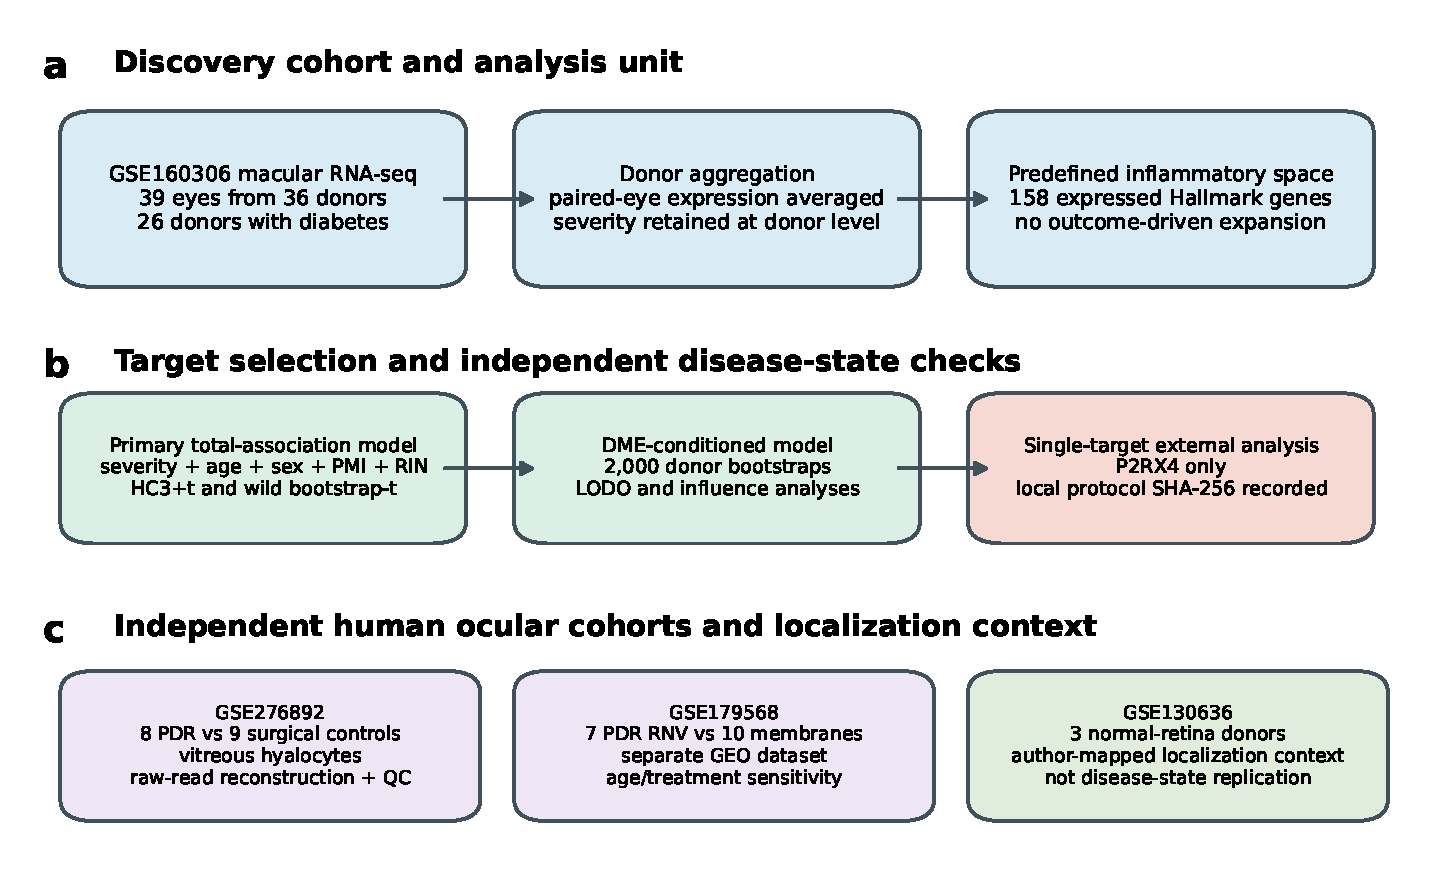
\includegraphics[width=\textwidth]{../figures/Figure_1_final_study_design.pdf}
\caption{Study design. (a) The donor, not the eye, is the biological unit in the GSE160306 discovery analysis. (b) P2RX4 was selected by the two-estimand severity analysis and locally specified as the only external target. (c) Separate human PDR-associated ocular datasets provide processed-value, raw-read, clinical-confounding, and direction sensitivities; GSE130636 supplies normal-retina localization context only.}
\label{fig:design}
\end{figure}

\subsection{Expression processing and inflammatory search space}

GSE160306 macular $\log_2(\mathrm{CPM}+1)$ values were mapped from Ensembl identifiers to symbols. When multiple rows mapped to one symbol, the row with the highest across-sample mean was retained. The search space was the expressed intersection with the MSigDB Hallmark inflammatory-response set \citep{Liberzon2015}, giving 158 genes. Positive coefficients were ranked because the question concerned inflammatory activation; all positive and negative results are retained in the supplementary workbook.

For paired-eye donors, expression and severity values were averaged so the predictor summarized the same eyes as the expression outcome. This produced a value of 39 for one donor whose eye-specific deposited scores were 35 and 43; 39 is an arithmetic donor summary, not an original clinical category. Sensitivities used the worst-eye score, rank-transformed donor severity, and a three-level clinical-stage code (diabetes without DR, NPDR, PDR). The stage code ignored DME so that retinal severity and DME were not collapsed into one ordinal variable.

\subsection{Severity estimands and small-sample inference}

For gene $g$, the primary total-association model was
\[
z(E_g)=\beta_0+\beta_1z(S)+\beta_2z(A)+\beta_3M+\beta_4z(P)+\beta_5z(R)+\epsilon,
\]
where $S$ is donor-mean supplied DR severity, $A$ age, $M$ male sex, $P$ post-mortem interval, and $R$ RNA integrity number. It estimates the severity--expression association without conditioning on DME. The secondary DME-conditioned model added a binary DME term and estimates severity association among donors with the same observed DME status. Neither model is a causal effect.

Heteroskedasticity-consistent HC3 covariance was combined with residual-degrees-of-freedom $t$ inference. A two-sided studentized wild-bootstrap-$t$ sensitivity used 4,999 Rademacher-weighted null-residual replicates with HC3 residual scaling. Benjamini--Hochberg correction covered the 158 severity tests within each estimand. Conventional confidence intervals are model-based, not post-selection-adjusted intervals.

\subsection{Stability, influence, and severity sensitivity}

The total-association model was refitted in 2,000 stage-stratified donor bootstraps. For every gene we retained the coefficient median and 95\% percentile interval, rank median and 95\% interval, positive-direction frequency, and top-5, top-10, and top-20 frequencies. Leave-one-donor-out (LODO) refits retained coefficient ranges and rank ranges. Leverage was compared with $2p/n$; Cook's distance and the severity DFBETA were computed for displayed candidates. Sensitivities excluded all high-leverage donors, used Huber robust regression, and substituted worst-eye, rank-transformed, or stage-coded severity. A P2RX4 severity-by-DME interaction was exploratory.

\subsection{Clinical contrasts and prediction audit}

NPDR without DME versus diabetes without DR was the primary binary contrast family of 158 genes. Four clinically narrower comparisons were exploratory families. Each contrast has a within-contrast Benjamini--Hochberg adjustment, and a global 790-test adjustment is provided as a sensitivity. Estimable covariate-adjusted binary models used HC3+$t$ inference; the two-donor PDR group was not covariate-adjusted.

Classification was retained only as supplementary falsification. In leave-one-donor-out folds, gene ranking, covariate residualization, scaling, and logistic fitting were learned from training donors. Any DR versus diabetes without DR was the outcome. A covariate-only model was analysed in parallel. AUC, Brier score, and log loss are descriptive internal audits and are not clinical-performance estimates.

\subsection{Single-target external analyses and raw-read reconstruction}

P2RX4 was locally fixed as the only external target before inspection of the processed GSE276892 values. The protocol SHA-256 is {\footnotesize\texttt{FA0EBEEF\allowbreak E4570917\allowbreak 8E197B6F\allowbreak 0819F7AA\allowbreak 1E1692E5\allowbreak 0AA2C7F4\allowbreak 7E2601D7\allowbreak CA3C8EED}}. The hash authenticates the current file content but does not prove its creation time; no public preregistration or independently timestamped target lock is claimed. The protocol specified a disease-only negative-binomial model and one-sided Wald test, but did not specify FASTQ alignment or quantification choices. Because GEO deposited normalized values rather than the source integer matrix, exact reproduction of the source count model was unavailable, whereas a post-protocol raw-read reconstruction remained possible.

For the source-faithful GSE276892 reconstruction, 10 new GSE276892 runs and 21 GSE147657 lanes were aligned with STAR 2.7.8a and counted with featureCounts 2.0.1 against GENCODE GRCh38.p13 release 42. Lane counts were summed to 17 biological samples. The primary reconstruction used the all-regions genome and annotation; the primary-assembly pair was a reference sensitivity. PyDESeq2 0.5.2 fitted disease-only negative-binomial models with one- and two-sided Wald inference. Post-protocol sensitivities added age/sex, reused-control source, both sets of covariates, excluded the exceptionally low PDR\_S10 profile, or restricted controls to the two newly generated profiles. Spearman analyses related raw and size-factor-normalized P2RX4 to mapping, assignment, library, detected-gene, cell-count, RNA-concentration, and clinical measures. These analyses are protocol deviations because the FASTQ-to-count workflow was not locally specified in advance.

Processed GSE276892 values were also summarized with two-sided Mann--Whitney tests, Cliff's delta, 10,000-bootstrap intervals, LODO direction stability, and HC3/Huber source and age/sex sensitivities. GSE179568 and GSE94019 were added after the local protocol and are post-protocol secondary checks. For GSE179568, age, sex, diabetes type, lens status, previous vitrectomy, anti-VEGF exposure, and panretinal photocoagulation were restored from the source Supplementary Table 1. Log$_2$(normalized value+1) HC3 regressions, Huber regression, and two-sided Mann--Whitney tests were reported for RNV versus macular-pucker membrane, with macular-hole and pooled-control sensitivities. Lack of age common support precluded propensity weighting and makes adjusted coefficients extrapolative. GSE94019 summed six deposited P2RX4 transcript-abundance rows per sample without labelling their unspecified units counts or CPM. Three post-protocol primary comparisons were Holm-adjusted. A retrospectively reconstructed GEO/PubMed search log records included and excluded datasets, value-inspection status when known, and one primary comparison per included dataset; it is not represented as a contemporaneous registry.

\subsection{Normal-retina localization context}

GSE130636 cluster identities were mapped from Voigt et al. Fig. 1F \citep{Voigt2019}. The six donor-region libraries, rather than 8,217 cells, were the aggregation units. The descriptive atlas panel was the six-gene union of the total-association and DME-conditioned top-five sets (P2RX4, TLR2, CD82, NLRP3, FPR1, and SLC31A1); no atlas result contributed to candidate ranking. Expression and detection were summarized within author-mapped cell types, then averaged across regions within donor. Dominant type was recalculated in three leave-one-donor folds, and between-donor minimum--maximum ranges were retained as descriptive intervals. These analyses describe normal-retina localization and cannot establish the producing cell in DR.

\subsection{Reproducibility and AI-assisted technologies}

Python 3.10, pandas, NumPy, SciPy, statsmodels, scikit-learn, Matplotlib, and PyDESeq2 were used; exact versions are included in the package. STAR 2.7.8a and featureCounts 2.0.1 were used on Linux for raw-read reconstruction. Random procedures used seed 20260813. Scripts, tests, input hashes, derived tables, and figure sources are publicly available at \url{https://github.com/xumedlab/DRnet}. OpenAI ChatGPT/Codex assisted language editing, code organization, and reproducibility checks. It did not generate primary data or images; authors reviewed all analyses and take responsibility for the manuscript.

\section{Results}

\subsection{P2RX4 is the only rank-one candidate under both severity estimands}

In the total-association model, the five largest positive coefficients were P2RX4, TLR2, CD82, NLRP3, and FPR1 (Fig.~\ref{fig:association}; Table~\ref{tab:candidates}). P2RX4 ranked first ($\beta=0.688$, HC3+$t$ 95\% CI 0.298--1.078, $P=0.00149$; wild-bootstrap $P=0.0008$). No gene survived 158-test correction in either prespecified primary severity estimand (total-association P2RX4 FDR=0.195), and the smallest total-association wild-bootstrap FDR was 0.126. Thus nominal and bootstrap tests support an association signal, not discovery-wide confirmation.

Adding DME retained P2RX4 at rank 1 ($\beta=0.599$, $P=0.00798$) but changed candidate identity: SLC31A1 rose from rank 14 to rank 2, whereas TLR2 moved from rank 2 to rank 6. CD82's DME-conditioned interval crossed zero ($P=0.0618$). P2RX4, NLRP3, CD82, and FPR1 were shared between the two top-five sets; only P2RX4 had the same first rank. The severity-by-DME interaction for P2RX4 was imprecise and non-significant and is reported as exploratory.

\begin{table}[h!]
\caption{Primary total-association candidates and stability}
\label{tab:candidates}
\centering
\small
\begin{tabularx}{\textwidth}{lrrrrrrX}
\toprule
Gene & Rank & $\beta$ & HC3+$t$ $P$ & Wild $P$ & Boot top-5 & LODO top-5 & Interpretation\\
\midrule
P2RX4 & 1 & 0.688 & 0.00149 & 0.0008 & 0.617 & 1.000 & discovery-selected; external single target\\
TLR2 & 2 & 0.641 & 0.0120 & 0.0082 & 0.461 & 0.962 & total-association dependent\\
CD82 & 3 & 0.568 & 0.0156 & 0.0080 & 0.282 & 0.769 & cross-estimand secondary\\
NLRP3 & 4 & 0.545 & 0.00310 & 0.0032 & 0.196 & 0.577 & cross-estimand secondary\\
FPR1 & 5 & 0.531 & 0.00448 & 0.0034 & 0.179 & 0.538 & cross-estimand secondary\\
SLC31A1 & 14 & 0.454 & 0.164 & 0.230 & 0.131 & 0.038 & DME-conditioned dependent\\
\bottomrule
\end{tabularx}
\end{table}

\begin{figure}[h!]
\centering
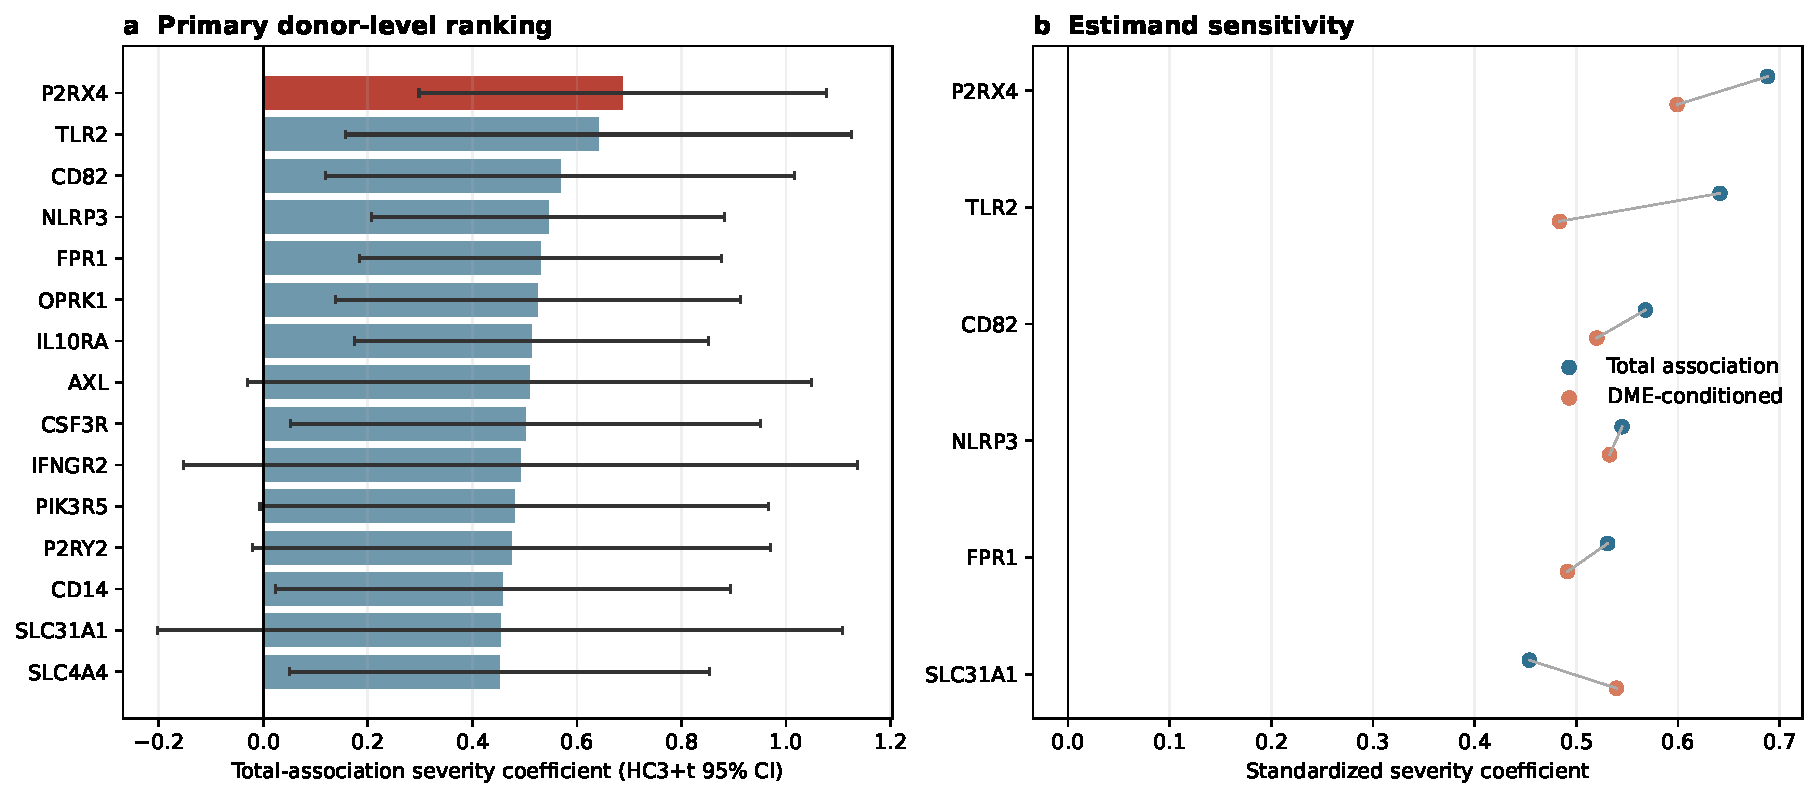
\includegraphics[width=\textwidth]{../figures/Figure_2_total_and_dme_conditioned_associations.pdf}
\caption{Severity estimands. (a) Top total-association coefficients with HC3+$t$ 95\% intervals. (b) Coefficients for the union of the two top-five sets under total-association and DME-conditioned models. These intervals are not selection-adjusted.}
\label{fig:association}
\end{figure}

\subsection{Resampling and influence analyses narrow the candidate claim}

P2RX4 appeared among the first five in all 26 donor-deletion refits, with a coefficient range of 0.591--0.753. Its 2,000-bootstrap top-five frequency was lower (61.7\%), however, with median rank 4 and a 95\% rank interval of 1--36 (Fig.~\ref{fig:stability}). TLR2 had bootstrap top-five frequency 46.1\%. CD82, NLRP3, and FPR1 ranged from 17.9\% to 28.2\%, showing that their apparent deletion stability did not translate into strong resampling identity stability. SLC31A1 had a 13.1\% bootstrap top-five frequency and 3.8\% LODO frequency in the total-association model.

Donor \texttt{13\_030} had leverage 0.771, above the $2p/n=0.462$ threshold, and PMI 149 minutes. P2RX4 nevertheless remained rank 1 after its exclusion ($\beta=0.683$) and under Huber regression ($\beta=0.762$), worst-eye severity ($\beta=0.687$), and rank-transformed severity ($\beta=0.721$). The rank-transformed sensitivity was the only tested severity representation in which P2RX4 crossed the 0.05 FDR threshold (BH FDR=0.0458); the clinical-stage code placed P2RX4 second behind TLR2. These encoding-dependent results support P2RX4 priority but not a stable multi-gene signature or a model-invariant discovery.

\begin{figure}[h!]
\centering
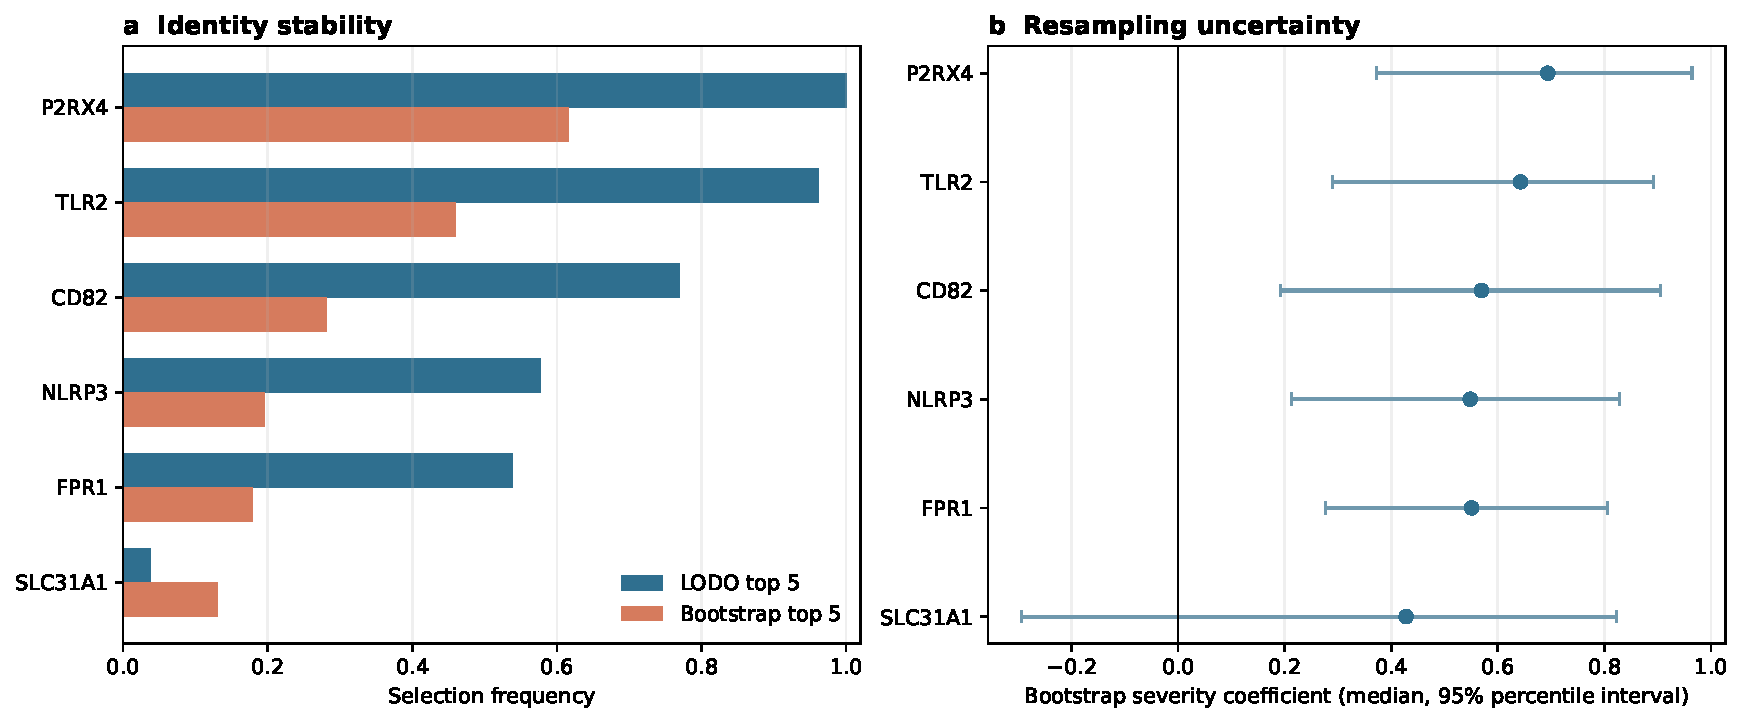
\includegraphics[width=\textwidth]{../figures/Figure_3_candidate_stability_and_uncertainty.pdf}
\caption{Ranking stability. (a) Top-five frequencies from donor deletion and stage-stratified bootstrap resampling. (b) Bootstrap coefficient medians and 95\% percentile intervals. The large difference between LODO and bootstrap identity frequencies motivates candidate tiering.}
\label{fig:stability}
\end{figure}

\subsection{External single-target checks are heterogeneous and confounded}

The locally specified GSE276892 comparison contained 8 PDR and 9 surgical-control profiles. In the post-protocol all-regions reconstruction, the disease-only P2RX4 negative-binomial estimate was positive but imprecise (log$_2$ fold change 0.295, 95\% CI $-0.854$ to 1.443; two-sided Wald $P=0.615$; one-sided $P=0.308$). The primary-assembly sensitivity was nearly identical (log$_2$ fold change 0.289; $P=0.622$). Source adjustment (log$_2$ fold change 0.808; $P=0.407$), source+age+sex adjustment (0.934; $P=0.417$), restriction to 8 PDR versus 2 newly generated controls (0.842; $P=0.506$), and exclusion of the exceptionally low PDR\_S10 profile (0.496; $P=0.105$) did not yield conclusive evidence. P2RX4 raw counts tracked assignment rate, mapping rate, total gene counts, and size factor; after normalization, P2RX4 was inversely correlated with detected genes (Spearman $\rho=-0.591$, BH-adjusted $P=0.0451$), emphasizing residual QC dependence.

The deposited processed values likewise gave higher raw-scale central tendency and rank ordering in PDR (two-sided Mann--Whitney $P=0.0927$; Cliff's $\delta=0.500$), but the mean-difference bootstrap interval included zero and the log-scale covariate sensitivity was null (Fig.~\ref{fig:validation}a). Seven of nine controls were reused from GSE147657, so disease and source were strongly associated. The reconstruction therefore replaces ``not evaluable'' with an evaluable but post-protocol and inconclusive count analysis; it does not establish a separable GSE276892 disease effect.

In post-protocol GSE179568, the unadjusted RNV-versus-macular-pucker comparison favoured PDR (two-sided Mann--Whitney $P=0.00967$; Cliff's $\delta=0.743$; unadjusted HC3 $\beta=0.696$, $P=0.0315$). However, PDR patients were aged 20--60 years and controls 62--83 years, leaving no observed age common support; the age standardized mean difference was $-2.83$. The age/sex-adjusted HC3 estimate was attenuated ($\beta=0.102$, $P=0.773$), the Huber estimate was similarly null ($\beta=0.202$, $P=0.570$), and the age/sex/treatment sensitivity was non-significant ($\beta=0.464$, $P=0.114$). These coefficients require extrapolation and cannot distinguish age, disease, treatment, or the markedly different membrane cell compositions. In GSE94019, the deposited 9 PDR and 4 control profiles had a positive mean direction but a non-significant two-sided Mann--Whitney $P=0.245$ (Fig.~\ref{fig:validation}c). Thus the external datasets offer heterogeneous, anatomically non-equivalent observations rather than independent disease-state replication.

\begin{figure}[h!]
\centering
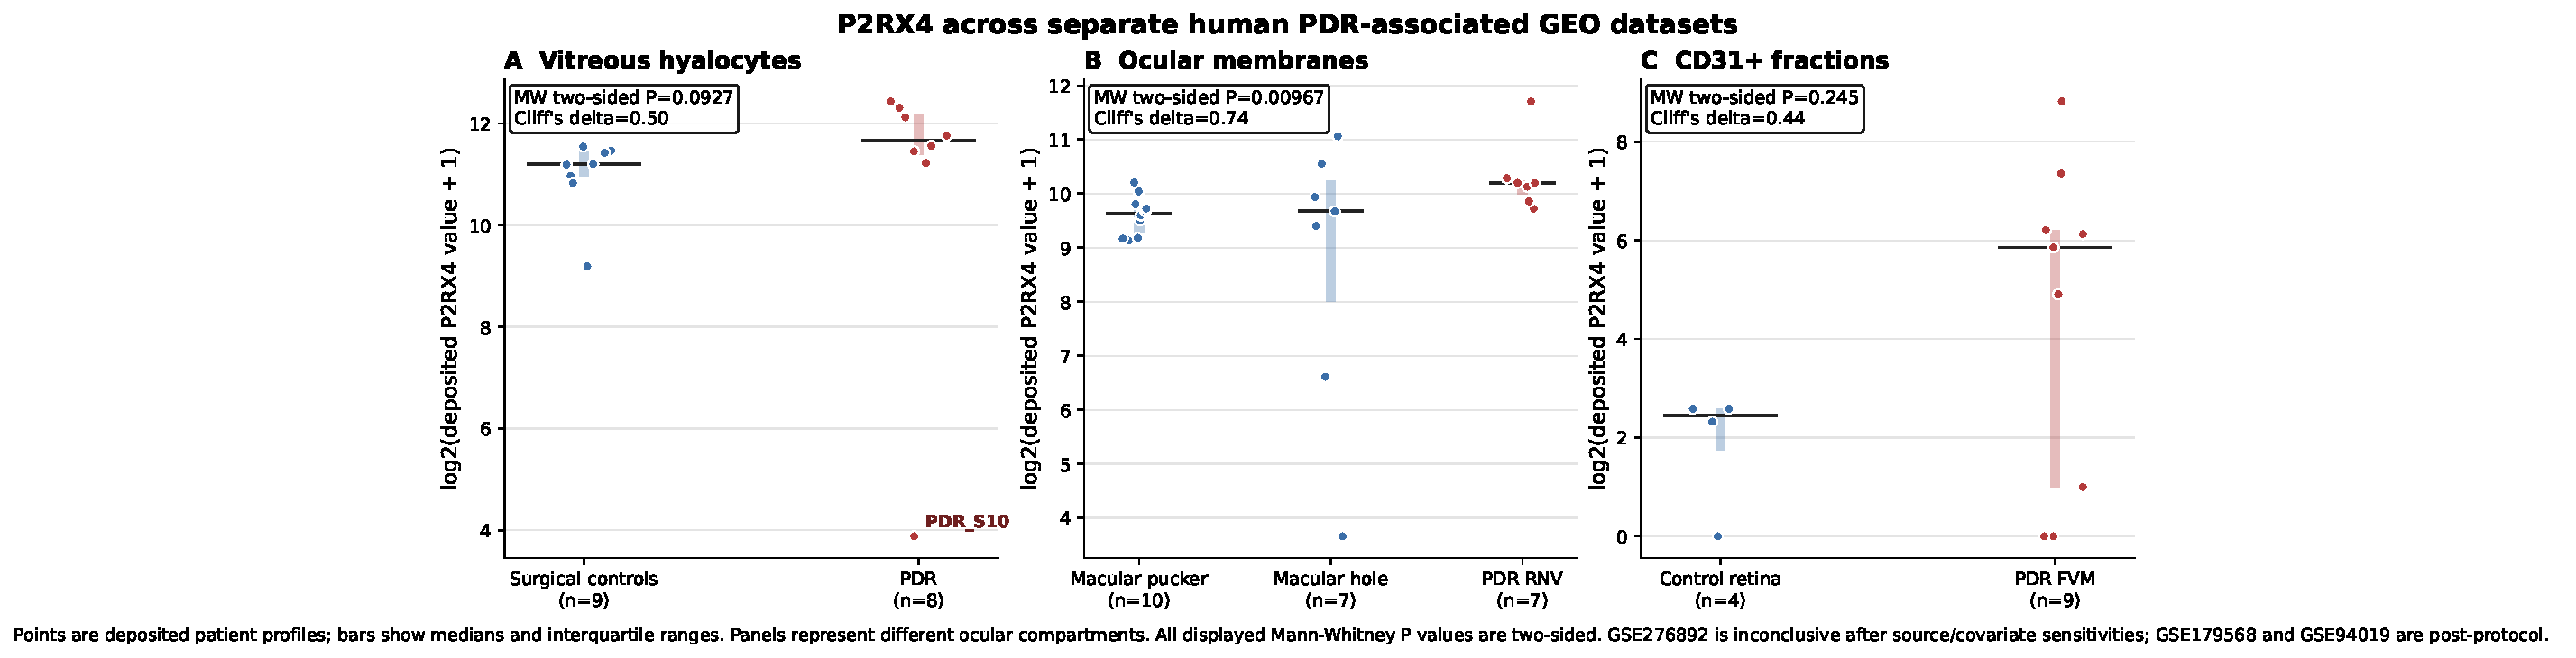
\includegraphics[width=\textwidth]{../figures/Figure_4_independent_P2RX4_validation.pdf}
\caption{Processed-value P2RX4 distributions in separate human PDR-associated GEO datasets. Points are deposited patient profiles; horizontal bars show medians and vertical bars show interquartile ranges on the log$_2$(deposited value+1) display scale. Displayed Mann--Whitney $P$ values are two-sided and operate on ranks, whereas raw-scale means/medians and log-scale regression answer different questions. (a) GSE276892 vitreous hyalocytes, with the exceptionally low PDR\_S10 profile labelled. (b) GSE179568 ocular membranes; these are a membrane-compartment comparison, not matched tissues. (c) GSE94019 CD31+ fractions. Raw-count reconstruction and clinical-confounding sensitivities appear in the Supplementary Information.}
\label{fig:validation}
\end{figure}

\subsection{Normal-retina localization is donor dependent for P2RX4}

In pooled GSE130636 normal-retina summaries, P2RX4 had its highest mean abundance in microglia, but this dominant type was retained in only one of three leave-one-donor folds (Fig.~\ref{fig:localization}). The other two folds were amacrine-dominant, and one dominance margin was nearly zero. By contrast, TLR2, NLRP3, and FPR1 were microglia-dominant in all three folds; CD82 was M\"uller-enriched-glia dominant in all folds; SLC31A1 was endothelial-dominant in two. These normal-retina patterns are localization context only and do not assign the PDR signal to a cell type.

\begin{figure}[h!]
\centering
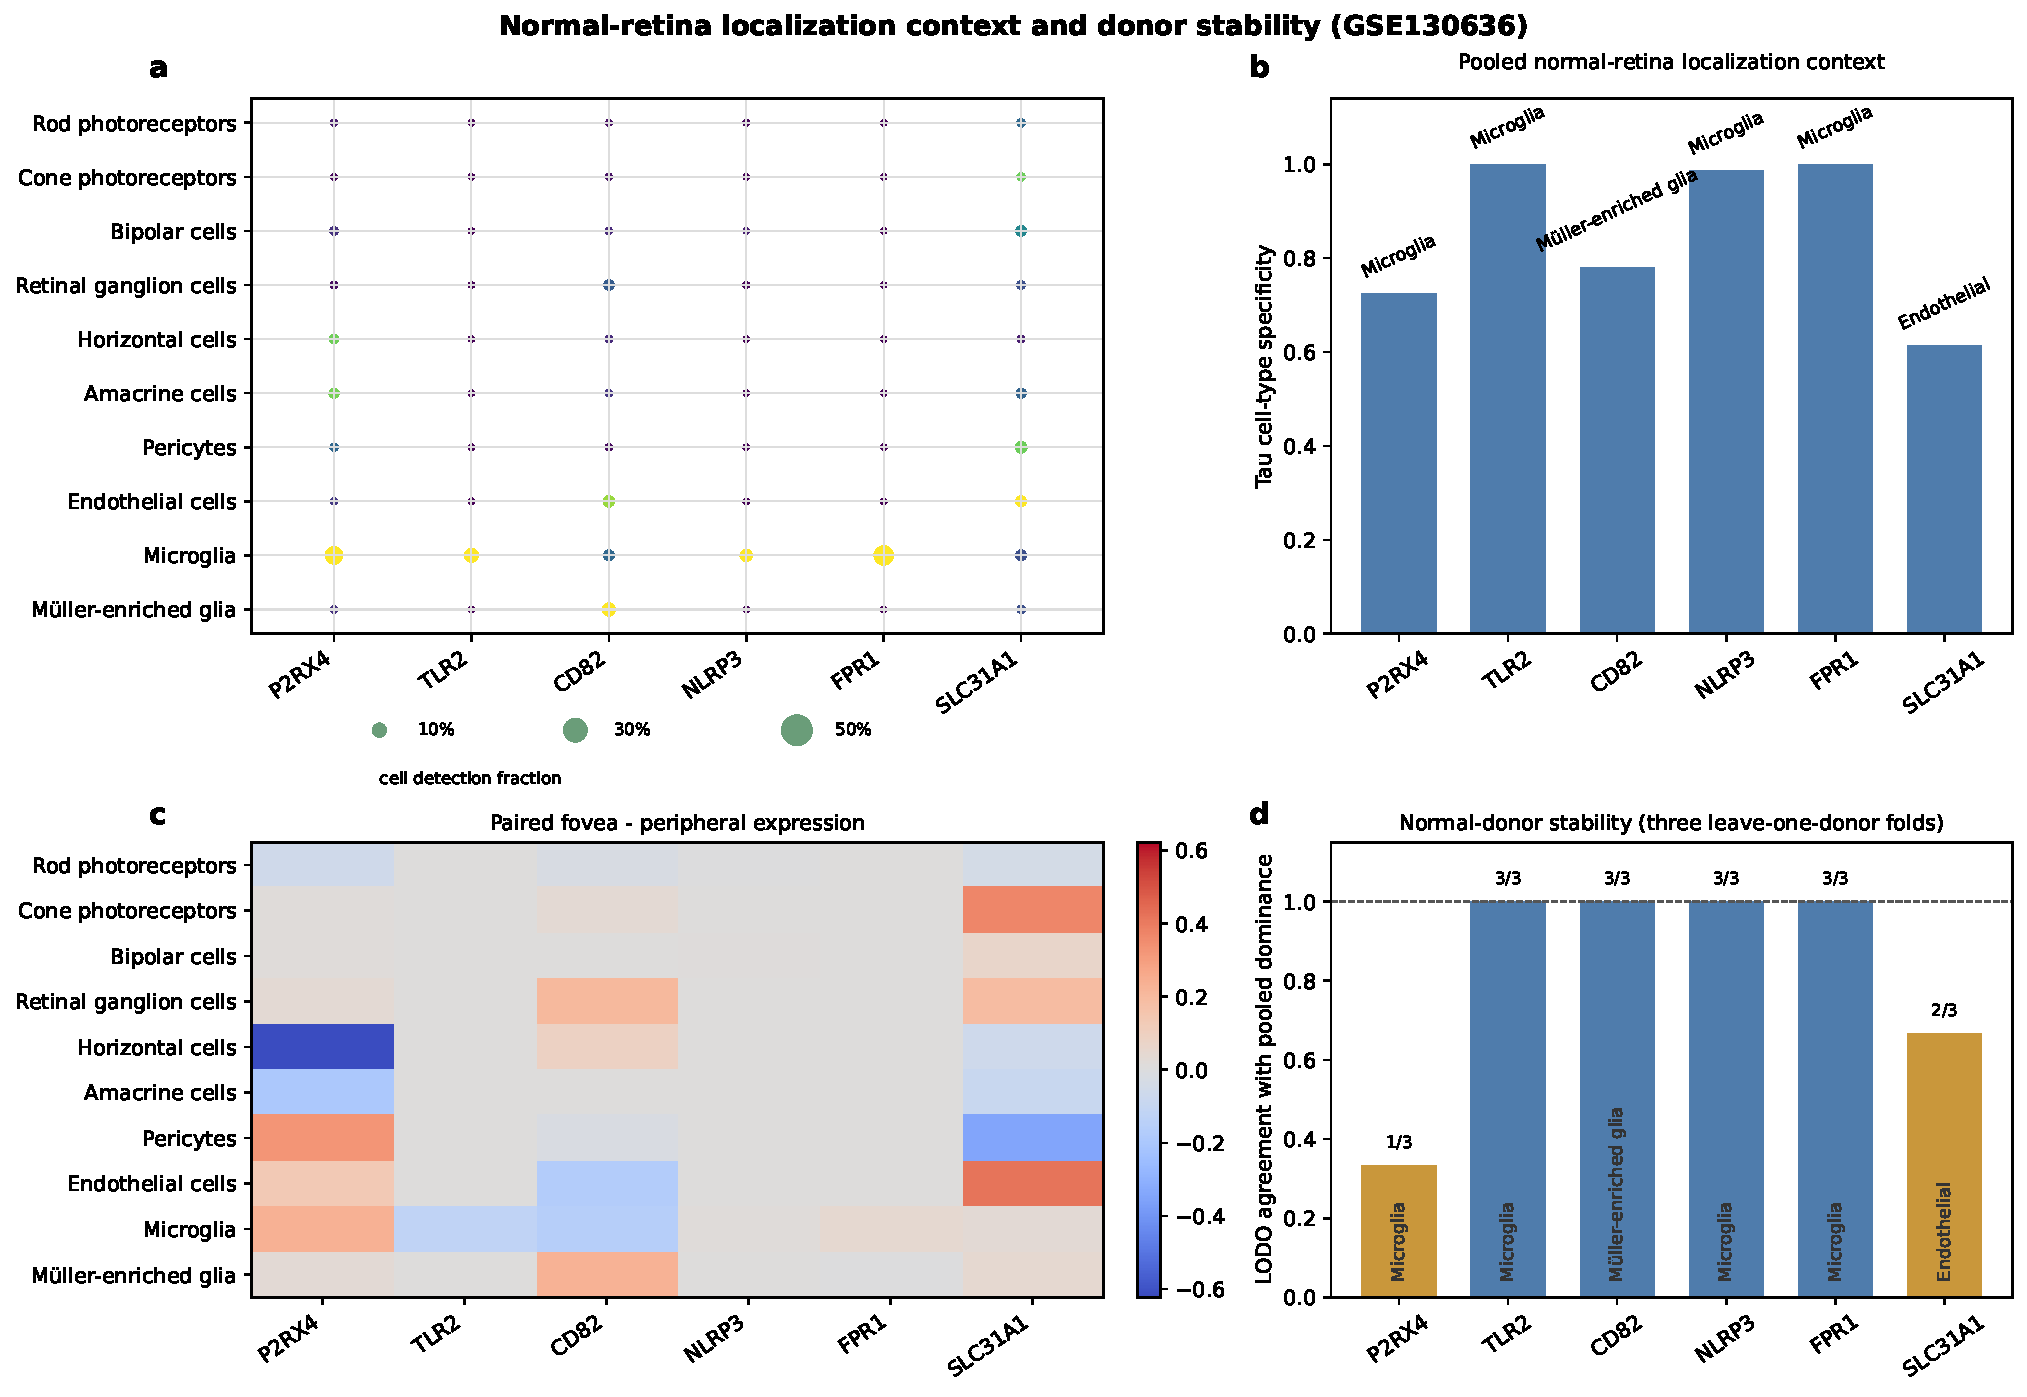
\includegraphics[width=\textwidth]{../figures/Figure_5_cell_type_localization.pdf}
\caption{Normal-retina localization context in GSE130636. (a) Mean abundance and detection by author-mapped cell type. (b) Pooled specificity. (c) Paired fovea--periphery differences across three donors. (d) Agreement of leave-one-donor dominant types with the pooled dominant type.}
\label{fig:localization}
\end{figure}

\subsection{Clinical contrasts and prediction remain supplementary}

The primary NPDR-without-DME versus diabetes-without-DR contrast was directionally positive for P2RX4. Across the five contrast families, no inference is promoted on the basis of a within-family nominal result; both within-contrast and global 790-test adjustments are available. The nested five-gene audit had AUC 0.681, Brier score 0.271, and log loss 0.935, whereas the covariate-only model had AUC 0.469, Brier score 0.272, and log loss 0.752. These unstable internal metrics do not support predictive claims and are omitted from the abstract.

\section{Discussion}

This study converts an internal inflammatory prioritization into a cross-cohort, single-target stress test. P2RX4 was the only candidate ranked first under both total-association and DME-conditioned severity models. It remained first after deleting the high-leverage donor, under Huber regression, and with worst-eye or rank-transformed severity, although its bootstrap identity stability was moderate and the stage code placed it second. The external analyses did not deliver clean replication: GSE276892 raw-count effects were positive but imprecise under every tested model, whereas the strongest GSE179568 processed-value contrast was severely age- and composition-confounded. The advance is therefore a donor-level human macular prioritization followed by transparent single-target ocular-compartment testing, including an inconclusive raw-read reconstruction, rather than a claim that P2RX4 is newly or definitively linked to DR.

The result is deliberately narrower than a conventional ``validated biomarker'' claim. No discovery gene survived FDR in either prespecified primary estimand, although P2RX4 crossed FDR=0.05 in the rank-transformed severity sensitivity. Its bootstrap top-five frequency was 61.7\%, and its bootstrap rank interval was broad. The source-reported P2RX4 results in GSE276892 and the PDR-versus-ILM comparison in GSE179568 did not survive their source analyses' across-gene adjustments. GSE179568 and GSE94019 were selected post-protocol, and contemporaneous records do not establish whether P2RX4 values were unseen at dataset selection. They are therefore exploratory observations rather than confirmatory support. P2RX4 should be considered a prioritized hypothesis, not a replicated effect or diagnostic signature.

The separation of DME estimands also changes interpretation. Without DME, TLR2 ranked second and SLC31A1 fourteenth. Conditioning on DME moved SLC31A1 to second and TLR2 to sixth. Because the data do not identify whether DME is a confounder, mediator, or consequence, neither result should be treated as the uniquely correct causal effect. Reporting both exposes model dependence and prevents a DME-conditioned coefficient from being mislabeled as overall DR progression.

The external compartments are both a strength and a limitation. Hyalocytes occupy the posterior vitreous cortex adjacent to the retina and RNV, whereas RNV and fibrovascular membranes contain mixtures of endothelial, myeloid, and stromal cells. Higher tissue-level P2RX4 can reflect within-cell regulation, altered cell composition, inflammatory-cell accumulation, technical source effects, or combinations thereof. It does not reproduce macular neurosensory retina. The GSE130636 atlas likewise cannot resolve this ambiguity: pooled P2RX4 localization was microglial, but donor deletion revealed instability. The appropriate conclusion is anatomically bounded ocular-compartment observation, not microglial exclusivity or a cell-intrinsic disease effect.

P2RX4 encodes the ATP-gated P2X4 receptor, which must be distinguished from the related P2RX7/P2X7 receptor and from receptor activity itself. In human umbilical-vein endothelial cells, high glucose plus palmitate increased P2X4 and P2X7 transcript and protein abundance; pharmacological and siRNA experiments implicated both receptors in parts of the inflammatory and permeability response \citep{Sathanoori2015}. This supplies biological plausibility but is not retinal evidence: HUVEC perturbation does not establish a retinal cell source, bulk P2RX4 mRNA does not measure channel activation, and tissue-level abundance can change through cell composition. The present innovation is therefore the donor-aware human macular prioritization and single-target external analysis, not the first association of P2X4 biology with diabetic stress.

Recent experimental work also provides context for secondary signals. In diabetic model systems, pharmacological disruption of uPAR/FPR1 signalling reduced retinal inflammation, blood--retinal barrier leakage, and functional impairment \citep{Canovai2026}; microglial AMPAR remodelling was linked to P2X7R/NLRP3/IL-1$\beta$ signalling and inner-barrier injury, with complementary measurements in human diabetic retina and vitreous \citep{Zhang2026NLRP3}; and STAT1-dependent SLC31A1 induction promoted cuproptosis-associated inflammatory microglial polarization in cells and diabetic mice \citep{Huang2026SLC31A1}. These studies increase mechanistic plausibility, but they neither validate the present human single-gene associations nor identify the cell type generating the bulk-tissue signal.

Other limitations include only 26 discovery donors, two PDR+DME donors, non-equidistant severity codes, three normal-retina atlas donors, source and QC dependence in GSE276892, absent age overlap and major tissue-composition differences in GSE179568, and tissue mismatch in GSE94019. The raw-read reconstruction used source-faithful software and annotation but remains post-protocol because the alignment and quantification workflow was not prespecified. The local protocol hash proves content identity, not timing. Different GEO accessions also do not prove patient non-overlap between the Freiburg datasets; public metadata were insufficient and no author confirmation was obtained. A genuinely separate human DR neurosensory-retina bulk or donor-pseudobulk single-nucleus cohort remains the most valuable next validation.

In conclusion, donor-aware, two-estimand analysis identifies P2RX4 as the highest-priority inflammatory candidate under the specified analyses in GSE160306. External analyses are directionally compatible in several raw-scale summaries but become inconclusive under the reconstructed negative-binomial and clinical-confounding sensitivities. The work supports P2RX4 as a focused hypothesis for genuinely independent retinal-cohort and experimental follow-up while quantifying why the present data do not constitute replication, cellular assignment, or mechanism.

\section*{Data availability}
All datasets analysed or audited are public in GEO: GSE160306, GSE276892, GSE147657, GSE179568, GSE94019, GSE130636, and GSE102485 \citep{GSE160306,GSE276892,GSE147657,GSE179568,GSE94019,GSE130636,GSE102485}. Raw-read accessions, reconstructed counts, derived patient-level tables, eligibility decisions, protocol deviations, clinical-covariate transcription, and input SHA-256 hashes are documented in the public reproducibility materials.

\section*{Code availability}
Project name: DRnet P2RX4 cross-cohort analysis. Operating systems: platform-independent Python analysis plus Linux raw-read reconstruction. Programming language: Python 3.10. Analysis code, tests, frozen analysis inputs, reconstructed-count summaries, derived tables, figures, environment records, and input hashes are publicly available at \url{https://github.com/xumedlab/DRnet}. The repository URL is stated without an unverified release tag, commit identifier, DOI, or licence claim.

\section*{Acknowledgements}
The authors thank the investigators and donors who made the GEO datasets available.
\section*{Funding}
The authors declare that no funds, grants, or other support were received during the preparation of this manuscript.
\section*{Author contributions}
MW and XZ contributed to study design, data analysis, and manuscript drafting. XS and PM contributed to interpretation, manuscript revision, and final approval. All authors read and approved the final manuscript.
\section*{Competing interests}
The authors declare no competing interests.
\section*{Ethics approval and consent to participate}
This secondary analysis used only de-identified public transcriptomic data and involved no new recruitment, tissue collection, animal experiment, or intervention. No additional institutional ethics approval was required for the computational reanalysis. The original studies reported their own ethical procedures.
\section*{Consent for publication}
Not applicable.
\section*{Supplementary information}
Supplementary Tables S1--S28 are provided in one workbook. The Supplementary Information contains expanded statistical methods, complete model and external-analysis results, raw-read reconstruction and QC, GSE179568 clinical-confounding analyses, influence and multiplicity analyses, normal-retina donor-stability analyses, predictive falsification, and the reproducibility inventory.

\bibliographystyle{sn-nature}
\bibliography{discover_references}
\end{document}
